\documentclass[a4paper, german, oneside]{scrbook}

\usepackage[german]{babel} %ngerman

\usepackage[utf8]{inputenc} 

\usepackage[T1]{fontenc}  
\usepackage{lmodern}

\usepackage{graphicx}

\usepackage{datetime}
\newdate{date}{15}{07}{2014}
\date{\displaydate{date}}

% Fußnote für Tabellen
\usepackage{tablefootnote}
\usepackage{amsmath}

% Auflistung in Text mit \begin{inparaenum}[(i)] und dann \item
\usepackage{paralist}
% Bessere Formatierung für Tabellen
\usepackage{booktabs}

% befehl: smaller, für relative schriftgröße
\usepackage{relsize}

\usepackage[babel,german=quotes]{csquotes}  % Deutsche Anführungszeichen mit \enquote{}

\usepackage[nottoc]{tocbibind}
\usepackage[style=authoryear, backend=biber, firstinits=false]{biblatex} % firstinits kürzt die Vornamen ab
\addbibresource{lit_ba_arbeit.bib}

\DefineBibliographyStrings{english}{andothers={et\ al\adddot}} % "u.a." zu "et al." 
% \DefineBibliographyStrings{english}{bibliography = {References}}
\DefineBibliographyStrings{german}{bibliography = {Literaturverzeichnis}}

% Internetquellen und sonstige Quellen separat
\defbibheading{LV}{\section*{Literaturverzeichnis}}
\defbibheading{IQ}{\section*{Internetquellen}}
 
\defbibfilter{LV}{\not\keyword{Internet}}
\defbibfilter{IQ}{\keyword{Internet}}
 


%richtige Reihenfolge bei mehreren Autoren
\DeclareNameAlias{sortname}{last-first}

%keine Klammern in Biblio
\renewbibmacro*{date+extrayear}{%
  \iffieldundef{year}
    {}
    {\printtext{\printdateextra}}}

\renewcommand*{\mkbibnamefirst}[1]{#1\addcomma} % #1 

% Commands für Textcite und Parencite mit Dropdownmenü
\newcommand{\citet}[1]{\textcite{#1}} 
\newcommand{\citep}[1]{\parencite{#1}}

% fix weird problem with unicode
\DeclareUnicodeCharacter{00A0}{ }


%%%%%%%%%%%%%%%%%%%%%%%%%%%%%%%%%%%%%%%%%%%%%%%%%%% Zitieren %%%%%%%%%%%%%%%%%%%%%%%%%%%%%%%%%%%%%%%%%%%%%%%%%%

% % Blockzitat mit Anführungszeichen
% \renewcommand*{\mkblockquote}[4]{\enquote{#1}#2#4#3}

% Blockzitat etwas kleiner
\newenvironment*{smallquote}
  {\quote\smaller}
  {\endquote}

% Now we instruct csquotes to use the new environment:

\SetBlockEnvironment{smallquote}
%%%%%%%%%%%%%%%%%%%%%%%%%%%%%%%%%%%%%%%%%%%%%%%%%%


\begin{document}
	\begin{titlepage}
	
		\begin{center}


		% Oberer Teil der Titelseite:
		% \includegraphics[width=0.15\textwidth]{./logo}\\[1cm]    

		\textsc{\LARGE Universität für Musik und Darstellende Kunst Graz}\\[1.5cm]

		% Titel der LV
		% \textsc{\Large Multivariate Datenanalyse (SS 2014)}\\[0.5cm]


		% Title
		\newcommand{\HRule}{\rule{\linewidth}{0.5mm}}
		\HRule \\[0.4cm]
		{ \huge \bfseries Das Publikum klassischer Konzerte}\\[0.4cm]

		\HRule \\[0.5cm] % Bei Untertitel auf 0.5 zurücksetzen


		\Large Kontinuitäten und Veränderungen seiner Zusammensetzung sowie der Bedeutung des Konzertbesuchs für das Bürgertum\\[2cm]
		% Evtl Wortumfang der Arbeit hier einfügen

		\Large \emph{Autor}:\\
		Thomas \textsc{Klebel}\\[0.1cm]
		\large 1073073\\[1cm]

		\Large \emph{Betreuerin:}\\
		Christa \textsc{Brüstle}\\[1cm]

		% \includegraphics[scale=0.5]{uni-graz_color.jpg}\\[1cm]    


		\vfill

		% Unterer Teil der Seite
		\Large{\today}\\[1cm]
		\normalsize{Zeichensatz mit \LaTeX}
		

		\end{center}

	\end{titlepage}

	
%%%%%%%%%%%%%%%%%%%%%%%%
% zähle die Titelseite nicht für die Seitenzahl
\clearpage
\setcounter{page}{1}
%%%%%%%%%%%%%%%%%%%%%%

\tableofcontents

\chapter*{Einleitung}
\addcontentsline{toc}{chapter}{Einleitung}
Die vorliegende Arbeit beschäftigt sich mit den Publika von klassischen Konzerten in Vergangenheit und Gegenwart. Um die Bedeutung des Konzertes für bestimmte Personengruppen, und die Zusammensetzung seines Publikums besser verstehen zu können, scheint es wichtig, einen Blick auf die Anfänge des \enquote{bürgerlichen Konzerts} zu werfen. Folglich widmet sich der erste Teil der Arbeit der Entwicklung des klassischen Konzerts, insbesondere im 19. Jahrhundert. Die Darstellung wird sich an folgenden Fragestellungen orientieren:

\begin{itemize}
	\item Welche Rolle spielte das Konzert im Leben der Bevölkerung des 19. Jahrhunderts? %viel zu allgemein
	\item Wie stellt sich das Verhältnis zwischen Konzertbesuch und sozialer Lage im 19. Jahrhundert dar?
	\item Gibt es verbindende Merkmale, die den KonzertbesucherInnen des 19. Jahrhunderts gemein sind?
\end{itemize}

Im zweiten Teil der Arbeit soll der/die LeserIn zu Beginn in die Theoriewelt Bourdieus eingeführt werden. Durch die Begriffe aus Bourdieus Gedankenwelt soll der Versuch unternommen werden, die Bedeutung des Konzertes für die Oberschicht des 19. Jahrhunderts zu untersuchen und die sozialen Praktiken der Distinktion offenzulegen.

Im weiteren Verlauf werden aktuelle empirische Daten zu den Konzertpublika dargestellt, um ein Bild über ihre Zusammensetzungen zu erhalten. Die Erkenntnisse aus der Untersuchung des Konzertpublikums des 19. Jahrhunderts sollen den empirischen Befunden über das heutige Konzertpublikum gegenüber gestellt werden:

\begin{itemize}
	\item Aus welchen Personen(gruppen) setzt sich das heutige Konzertpublikum zusammen?
	\item Welche Gemeinsamkeiten und Unterschiede lassen sich im Vergleich mit dem Konzertpublikum des 19. Jahrhunderts finden?
\end{itemize}

Vorweg bedarf der Terminus des \emph{klassischen} Konzerts einer kurzen Eingrenzung. Dem allgemeinen Sprachgebrauch in der Musikwelt entsprechend wird in der vorliegenden Arbeit unter dem klassischen Konzert ein öffentliches Konzert verstanden, bei dem Werke, die von der Epoche des Barock bis zur \enquote{neuen Musik} des 20. Jahrhunderts reichen, in nicht-szenischer, also konzertanter Form aufgeführt werden. 

%%%%%%%%%%%%%%%%%%%%%%%%%%%%%%%%%%%%%%%%%%%%%%%%%%%%%%%%%%%%%%%%%%%%%%%%%%%%%%%%%%%%%%%%%%%%%%%%%%%%%%%%%%%%%%%%%%%%%%%%%%%%%%%%%%%%%%%%%%%%%%%%%%%%%%%%%%
%%%%%%%%%%%%%%%%%%%%%%%%%%%%%%%%%%%%%%%%%%%%%%%%%%%%%%%%%%%%%%%%% Historischer Teil %%%%%%%%%%%%%%%%%%%%%%%%%%%%%%%%%%%%%%%%%%%%%%%%%%%%%%%%%%%%%%%%%%%%%%
%%%%%%%%%%%%%%%%%%%%%%%%%%%%%%%%%%%%%%%%%%%%%%%%%%%%%%%%%%%%%%%%%%%%%%%%%%%%%%%%%%%%%%%%%%%%%%%%%%%%%%%%%%%%%%%%%%%%%%%%%%%%%%%%%%%%%%%%%%%%%%%%%%%%%%%%%%


\part{Historischer Teil}

\chapter{Einleitung}
Um die Zusammensetzung des heutigen Konzertpublikums zu untersuchen erscheint es sinnvoll, zuerst einen Blick auf die Genese des Konzerts zu werfen: Wann ist das Konzert, so wie wir es heute kennen, entstanden? Aus welchen Formen ist es entstanden, welche Vorläufer gab es? Auf Basis der Antworten auf diese Fragen lassen sich dann die heutigen Entwicklungen diskutieren.

Um einen guten Überblick über die Genese des Konzerts zu bieten, wird im folgenden das Musikleben des 19. Jahrhundert von unterschiedlichen Blickwinkeln aus betrachtet. Neben einem kurzen historischen Überblick über die wichtigsten Geschehnisse dieses Jahrhunderts sollen hauptsächlich die für die Entstehung des \enquote{bürgerlichen} Konzerts bedeutenden Formen dargestellt werden: 
\begin{inparaenum}[(1)]
	\item das Liebhaberkonzert, 
	\item die geschlossene Konzertvereinigung, sowie 
	\item die professionelle Konzertgesellschaft.
\end{inparaenum}

In der Folge wird auf einen wichtigen Motor für die Entwicklung des Konzerts eingegangen, die Professionalisierung des Konzertbetriebs. Zuletzt soll ein Blick auf den Lebensstil und die soziale Zusammensetzung des Publikums geworfen werden.


% \chapter{Das Musikleben im 18. Jahrhundert}
% \label{18jh}
% Mix aus verschiedenen Stücke, arien etc (Weber: 3)

% Aus heutiger PErspektive erstaunlich erscheint die Tatsache, dass das Liebhaberkonzert im Grunde ein Potpourri aus den verschiedensten WErken war. Typischerweise eröffnete es mit einem Satz aus einer Sinfonie, auf den Lieder, Arien, und virtuose Instrumentalstücke folgten. (Literatur!!!)



\chapter{Das Musikleben im 19. Jahrhundert}
\label{19jh}

\section{Historischer Überblick: Das 19. Jahrhundert}
\label{histUberblick}
Bei der Untersuchung der Musik und des Publikums lassen sich die historischen Ereignisse der Zeit nicht ignorieren, sie bilden vielmehr den Rahmen für alle Entwicklungen, die im weiteren Verlauf behandelt werden sollen. Insofern erscheint es angeraten, an den Anfang der Untersuchungen über das Musikleben im 19. Jahrhundert einen kleinen historischen Überblick zu geben, der sich, ob des Rahmens der Arbeit, beispielhaft auf die wichtigsten Ereignisse konzentrieren wird.

Kalendarisch reichte das 19. Jahrhundert von 1801-1900. Trotzdem scheint es angebracht, den Rahmen etwas zu erweitern. Durch die Einbeziehung der französischen Revolution lässt sich ein besseres Bild der Entwicklungen darstellen.

Ausgehend von der französischen Revolution 1789 entwickelte sich Europa weg von monarchistischen Reichen, hin zu demokratischen Nationalstaaten. Nachdem auf die französische Revolution eine Zeit der Restauration folgte, gewann das Bürgertum mit den Revolutionen 1830 und 1848 deutlich an Einfluss. \parencite[vgl.][253ff.]{demandt_kleine_2003}

Ein Katalysator für den Aufstieg des Bürgertums war sicherlich die industrielle Revolution, und die daraus folgende Urbanisierung. Mit der Erfindung der Dampfmaschine im 18. Jahrhundert war der Grundstein für eine große Umwälzung der Wirtschaft, und in der Folge auch des Lebens der Menschen gelegt. Durch den Aufstieg der dampfgetriebenen Eisenbahn könnten Güter und Personen viel großräumiger bewegt werden. Insgesamt ging der Anteil der Beschäftigten im primären Sektor, der Agrar- und Landwirtschaft durch die technischen Fortschritte stark zurück, es entwickelte sich die \emph{Industriegesellschaft}. Sie war geprägt durch kapitalistische Warenproduktion. Die vom Land in die Städte ziehende Bevölkerung arbeitete unter schlechten Bedingungen in Fabriken, und trug, um mit Marx zu sprechen, zu einer Akkumulierung des Kapitals in den Händen der Unternehmer bei. (\cite{marx_kapital:_1989}; \cite[368]{hillmann_worterbuch_2007}) Der Aufstieg und die dadurch bedingte Eigenständigkeit des Bürgertums waren auch für die Entwicklungen im Musikleben bedeutend, wie wir in den nächsten Abschnitten sehen werden.


\section{Konzerttypen im 19. Jahrhundert}
\label{konzerttypen}
Die folgende Darstllung des Konzertpublikums orientiert sich an Webers Studie über die Konzertpublika der ersten Häfte des 19. Jahrhunderts. \citep{weber_music_2004} Weber spricht von Konzerten in der Sphäre der \enquote{popular music}, sowie von Konzerten der \enquote{classical music}. \enquote{Popular music} bezeichnet hier hauptsächlich Konzerte der zur damaligen Zeit erfolgreichen Virtuosen, welche ein breites Publikum anzogen. Webers Begriff der \enquote{benefit concerts} scheint am ehesten dem Begriff der Liebhaberkonzerte zu entsprechen, weswegen ich letzteren in der Folge synonym verwenden werde. 


\subsection{Das Liebhaberkonzert}
\label{liebhaber}
Obwohl der Terminus der \enquote{populären Musik} umstritten sein mag, so war doch das Liebhaberkonzert ein wichtiger Schritt auf dem Weg zur Form des Konzerts, so wie wir sie heute erleben. In der ersten Hälfte des 19. Jahrhunderts gehörte es zu einer Gemengenlage, die maßgeblich an der Erweiterung des Publikums beteiligt war. Zu dieser Gemengenlage gehörten unter anderem eine institutionalisierte Form von Salons und Konzerten, die zusammen mit dem aufkeimendem Unternehmertum und der Professionalisierung der MusikerInnen ein wachsendes Publikum aus der Aristokratie und der oberen Mittelschicht für sich gewinnen konnte.

Um die Rahmenbedinungen des Liebhaberkonzerts besser zu verstehen lohnt sich ein Blick in die Welt des Publikums dieser Konzerte.

Musik hatte für die aristokratischen Zirkel und die auf eine Verbesserung ihrer gesellschaftlichen Position bedachte obere Mittelschicht mehrere Funktionen. Ein erster Grund für die Tatsache, dass Musik eine immer wichtigere Rolle im Leben der Menschne einnahm war ihre Verankerung in der Familie. Zuerst einmal war eine musikalische Erziehung der Kinder ein guter Weg, sie Disziplin zu lehren: das Erlernen eines Musikinstruments fordert regelmäßige und konzentrierte Übung, folglich ein gewisses Maß an Dispziplin. \parencite[35ff.]{weber_music_2004} In der Folge waren musizierende Kinder auch ein probates Mittel, um in den Salons der Aristokratie einen guten Eindruck zu machen. Die Zusammenkünfte in den Salons waren in mehrerlei Hinsicht gesellschaftlich bedeutsam. Für junge, musizierende Mädchen war es mitunter ein guter Ort um Aufmerksamkeit auf sich zu lenken, die eventuell in einer Ehe mit einer bedeutenden Familie enden könnte. Auch die Zurschaustellung des eigenen Lebensstils, zum Beispiel durch die Wahl der Kleidung war ein wichtiger Bestandteil der Salons.\footnote{Auf die ---- des Lebenstils wird im Abschnitt \ref{lebensstil} eingegangen werden.} Nicht zuletzt war der Erweb musikalischer Fähigkeiten, um sich in den Salons der angesehenen Familien bewegen zu können, teilweise auch ein Weg zu einer guten Anstellung: \blockquote[{\cite[37]{weber_music_2004}}]{A correspondent to a Leipzig music magazine reported that in Vieanna young men took up chamber music in order to gain access to the salons of highly-placed families through whom they might get good jobs.}

Auch war die Rolle der Frauen in diesen Kreisen insgesamt eine sehr bedeutsame. Frauen waren nicht nur von klein auf musikalisch tätig, was sie auch oft nach der Hochzeit fortsetzten. Sie waren auch für das gesellschaftliche Familienleben im Allgemeinen zuständig: Frauen organisierten die Zusammenkünfte in den Salons, stellten die Gäste vor, und führten die Konversation. Auch die Tatsache, dass der Gesang und das Klavierspiel, zwei -- zumindest zur damaligen Zeit -- Domänen der Frauen, die beliebtesten musikalischen Formen in den Salons waren, spricht für die Bedeutung, die Frauen im musikalischen Leben der Familien spielten. \parencite[vgl.][41]{weber_music_2004}

Bei der Betrachtung der Musikszene in den Salons könnte der Gedanke aufkommen, Musik sei nur als Mittel zum Zweck, als Möglichkeit, seine gesellschaftliche Position zu verbessern zu verstehen gewesen. Das trifft bei den öffentlichen Konzerte aus einem einleuchtenden Grund nicht zu: während man in den privaten Kreisen der Salons noch leicht einen Überblick über die anwesenden Personen behalten konnte, war das aufgrund der größer werdenden Publika bei den öffentlichen Konzerten, und der allgemeinen Zunahme der öffentlichen Konzerte nicht mehr möglich. \parencite[vgl.][37]{weber_music_2004} Dies führt nun zur Frage, worauf diese Zunahme zurückzuführen ist. 

% nachfolgend einbinden, wie es im 18. Jh war, kein extra kapitel
Die frühen Formen des Konzerts im 18. Jahrhundert bestanden aus einem Potpourri von verschiedenen Stücken, Arien, Tänzen und virtuosen Stücken. Das Liebhaberkonzert hatte anfangs eine ähnliche Zusammensetzung. Ausgehend vom Virtuosenkult um Instrumentalisten wie Franz Liszt oder Niccolò Paganini veranstalteten einzelne MusikerInnen Konzerte, in denen sie sich präsentieren konnten. Diese Konzerte waren mit der den musikalischen Aktivitäten in den privaten Kreisen eng verzahnt: einerseits traten die Solisten in den Salons auf, um für Unterhaltung zu sorgen, sowie teilweise auch um mit Familien in Kontakt zu kommen, deren Kinder sie dann unterrichten konnten. Auf der anderen Seite wurde dann von den Gesellschaften, in die sie eingeladen worden waren, erwartet, dass diese das regelmäßig (zum Beispiel jährlich) stattfindende öffentliche Konzert des Virtuosen zu besuchen. Aus der Nennung von Liszt oder Paganini wird klar, was das Besondere an den Konzerten war: es ging zentral um die Präsentation eines oder mehrerer Virtuosen, die mit ihren ungeahnten Fähigkeiten auf dem Instrument die Menschen begeisterten. \parencite[vgl.][24]{weber_music_2004}

Trotzdem, und auch gerade weil die Konzerte eine große Anzahl an Menschen anzuziehen vermochten, entstand dadurch noch kein vereintes, elitäres Publikum, wie es später durch die Bildung von Symphonieorchestern verstärkt geschah. Durch die einzelnen MusikerInnen, die sich unternehmerisch betätigten, gab es eine solche Vielzahl an Konzerten, dass nicht alle von ihnen in der Lage waren, ein großes Publikum anzuziehen. In der Folge blieben die Konzertsäle oft teils leer, oder es wurden Karten zu geringen Preisen oder überhaupt gratis vergeben, um zumindest den Anschein eines großen Andranges zu erwecken. \parencite[vgl.][49ff.]{weber_music_2004}

Ungeachtet dieser Einschränkungen bildeten die Liebhaberkonzerte aber eine zentrale Rolle in der Entwicklung des modernen Konzerts. Einerseits legten sie den Grundstein für Konzertformen wie das heute praktizierte Recital. Andererseits schufen sie durch die Vielzahl an Institutionen und Gewohnheiten die sie begünstigten, wie das musikalische Verlagswesen, die Musikpresse, und die allgemeine kommerzielle Ausrichtung der Konzerte, die Grundlage für die weiteren Entwicklungen des Konzertwesens.

\subsection{Die geschlossene Konzertvereinigung}
\label{konzertvereinigung}

%fehlt: unterscheidung zwischen populärer und "klassischer" musik.  klar machen, dass bei weber liebhaberkonzerte in die erste Kategorie fallen.
Parallel zu den Entwicklungen im Rahmen der populären Musik entstanden im 19. Jahrhundert auch so genannte Konzertvereinigungen. Am Beispiel der \enquote{Ancient Concerts} und der \enquote{Royal Philharmonic Society} in London lässt sich deren Wesen erläutern.

Das Publikum der Ancient Concerts bestand anfangs fast ausschließlich aus Vertretern des hohen Adels und des Klerus. Nur auf Einladung durch die Direktoren, welche natürlich selbst dem hohen Adel angehörten, war es Personen gestattet, zu den Konzerten zu kommen. Entsprechend dem Geschmack der Elite wurden hauptsächlich Stück von Komponisten gespielt, die seit mindestens 20 Jahren verstorben waren. Faktisch bestand das Programm also aus Werken der Renaissance und des Barock. Im Lichte der zunehmenden Professionalisierung in anderen Bereichen des Musiklebens, sowie der steigenden Nachfrage nach \enquote{moderner} Musik, verlor die Konzertreihe allmählich an Reputation. (\cite[92ff.;]{muller_publikum_2014} \cite[73]{weber_music_2004})

Die Nachfrage des hohen Bürgertums nach aktuellerer Musik und größerer Unabhängigkeit von der Aristokratie wurde durch die Gründung der Royal Philharmonic Society, zumindest für eine kurze Periode, gestillt. Auch hier war die Mitgliedschaft nur durch die offizielle Aufnahme durch das Direktorium möglich. Im Gegensatz zu den Ancient Concerts machten Adlige hier aber den kleinere Teil aus. Der private Charakter der Veranstaltungen zeigte sich auch in der Tatsache, dass die Weitergabe der Eintrittskarten an Freunde strengstens untersagt war. \parencite[vgl.][93]{muller_publikum_2014}

Insgesamt war auch bei den geschlossenen Konzertvereinigungen die Tendenz der Professionalisierung zu beobachten. (vgl. Abschnitt \ref{professionalisierung}) Die Programme der Konzerte waren aber von denen der Liebhaberkonzerte grundverschieden. Während bei letzteren neue und virtuose Stücke für Begeisterung sorgten, waren es im Rahmen der Konzertvereinigungen und der noch zu besprechenden Konzertgesellschaften (vgl. Abschnitt \ref{konzertgesellschaft}) eher die \enquote{klassischen} Werke von Haydn, Mozart und Beethoven, die zur Aufführung gelangten. \parencite[vgl.][22f]{weber_music_2004}


\subsection{Die professionelle Konzertgesellschaft}
\label{konzertgesellschaft}
Aus den Konzertvereinigungen heraus entwickelten sich in der zweiten Hälfte des 19. Jahrhunderts Konzertgesellschaften, die immer professioneller organisiert wurden.\footnote{Der Prozess der Professionalisierung des Konzertbetriebes wird im nächsten Abschnitt besprochen.} Das Wesen der Konzertgesellschaften ähnelte schon sehr stark den heutigen Konzertgesellschaften (wie zum Beispiel der Grazer \emph{Musikverein für Steiermark} oder die \emph{Gesellschaft der Musikfreunde in Wien}). Die Zugehörigkeit zu der Gesellschaft war nicht mehr durch eine formelle Aufnahme beschränkt, es wurden vielmehr Eintrittskarten für eine Saison verkauft (Abonnement), im späteren Verlauf dann auch Einzelkarten. \parencite[vgl.][106]{heister_konzert:_1983}

Innerhalb dieser Konzertgesellschaften entstand auch eine zunehmende Kanonisierung des Repertoires: Die Sinfonie als gesamtes \emph{Werk} gewann an Bedeutung, sie wurde zum Kulminationspunkt der \emph{absoluten} Musik im Orchester. In der Folge ging auch die Praxis, nur einzelne Sätze aufzuführen deutlich zurück. \parencite[vgl.][231ff.]{muller_publikum_2014}



\section{Professionalisierung des Konzertbetriebs}
\label{professionalisierung}
Die Professionalisierung des Konzertbetriebs war ein bedeutender Schritt zur Entwicklung des modernen Konzertes. Für Symphonieorchester heute mehr oder weniger selbstverständlich Dinge wie ein/e DirigentIn oder mehrere Proben vor einer Aufführung waren im 19. Jahrhundert noch keine Selbstverständlichkeit. So war es beispielsweise üblich, dass die Leitung des Ensembles jeweils wechselte: jeweils unterschiedliche Musiker des Ensembles übernahmen für einzelne Konzerte die Leitung des Konzerts. \parencite[vgl.][68]{weber_music_2004} Alternativ war es auch möglich, dass entweder der/die KonzertmeisterIn oder auch der/die KomponistIn, zum Beispiel vom Klavier aus die Einsätze gab. Die Einführung einer fixen künstlerischen Leitung in Form eines/r DirigentIn führte verständlicherweise zu einer genaueren, ergo \enquote{besseren} Darbietung.\footnote{Die Fragen, was in diesem Zusammenhang als \enquote{gut} oder \enquote{besser} zu verstehen ist, ist beileibe keine eindeutige. Schon im 19. Jahrhundert war die Frage nach der \enquote{Werktreue} eine heiß diskutierte. Unstrittig bleibt aber, dass durch die Einführung eines/r DirigentIn im Orchester größere Ordnung herrschte, was der Qualität der Aufführungen, sofern man darunter eine akkurate Wiedergabe des Werkes versteht, sicherlich zuträglich war.}

Neben der \enquote{Erfindung} des/r DirigentIn (Müller) war auch die Einführung mehrerer Proben ein wichtiger Schritt, um das Niveau der Aufführungen zu heben. Nicht zuletzt durch die steigende Anzahl von Proben bestanden die Ensembles zunehmend aus professionellen MusikerInnen, welche als Hauptbeschäftigung der Musik nachgingen. Diese Feststellung ist deshalb wichtig, da in den Anfängen des Konzertbetriebes die musizierenden Personen meist Amateure waren: sie gingen hauptberuflich einer anderen Tätigkeit nach, und \enquote{dilettierten} in ihrer Freizeit.

Am Begriff des \emph{Dilettanten} lässt sich dieser Wandel leicht zeigen. Der Duden listet für das Wort \enquote{Dilettant} zwei Bedeutungen:
\begin{inparaenum}[(a)]
	\item jemand, der sich mit einem bestimmten [künstlerischen, wissenschaftlichen] Gebiet nicht als Fachmann, sondern lediglich aus Liebhaberei beschäftigt, sowie
	\item (abwertend) jemand, der sein Fach nicht beherrscht.
\end{inparaenum}
\parencite{Dilettant}

Besonders die abwertende Verwendung des Wortes scheint heute die geläufige zu sein. Ganz im Gegensatz dazu steht seine Konnotation im 19. Jahrhundert: Der in seiner Freizeit dilettierende Bürger galt quasi als Ideal. Besonders in Wien waren die dilettierenden Musiker von großer Bedeutung und bremsten somit die Professionalisierung. \parencite[vgl.][88]{weber_music_2004}


% Sitzplatznummerierung

\section{Der Lebensstil des Konzertpublikums} %ev: die soziale Zusammensetzung des Publikums?
\label{lebensstil}
Wie schon aus den vorangegangenen Kapiteln ersichtlich rekrutierte sich das Publikum von klassischen Konzerten zur damaligen Zeit hauptsächlich aus den Reihen der Aristokratie sowie der oberen Mittelschicht. Innerhalb der verschiedenen Konzerttypen lässt sich aber eine weitere Differenzierung des Bürgertums nach der Berufsgruppe vornehmen.

Weber spricht von Konzerten der \enquote{popular music}, den Liebhaberkonzerten auf der einen Seite und denen der \enquote{classical music} auf der anderen Seite. In beiden Bereichen war das Bürgertum vertreten, nur eben durch unterschiedliche Berufsgruppen. Während in den Konzerten der \enquote{popular music} eher Unternehmer und ihre Familien zu finden waren, schienen die Konzerte der \enquote{classical music} eher eine Domäne der freien Berufe und der Beamten, in weiterer Konsequenz also der Männer zu sein. \parencite[vgl.][S. 63 und 66]{weber_music_2004}

In Verbindung mit den Berufsgruppen stand auch ihr Lebensstil. Nach Weber interessierten sich die Unternehmersfamilien besonders stark für die Virtuosen der \enquote{popular music}, da diese ihrem Lebensstil entsprachen: \blockquote[{\cite[39]{weber_music_2004}}]{Most business families accordingly had a self-confident, ostentatious lifestyle and valued cultural pursuits of the same order. They looked to the famous virtuosi for an exaggerated picture of the success and glamour they saw in themselves.}

Die Tatsache, dass Vertreter der freien Berufe sowie der Beamtenschaft bei den Konzerten der \enquote{classical music} stark vertreten waren, liegt in der Ausbildung dieser Berufsgruppen begründet: für Berufe wie den des Arztes oder des Rechtsanwaltes war, genauso wie für die Aufnahme in den Staatsdienst, eine universitäre Ausbildung eine Voraussetzung. In der Ausübung und Wertschätzung der schon damals \enquote{klassischen} Musik konnten sie ihren intellektuellen Habitus ausspielen und ihren Status verbessern. \parencite[vgl.][67]{weber_music_2004}




% \section{Kanonbildung in der klassischen Musik}

%%%%%%%%%%%%%%%%%%%%%%%%%%%%%%%%%%%%%%%%%%%%%%%%%%%%%%%%%%%%%%%%%%%%%%%%%%%%%%%%%%%%%%%%%%%%%%%%%%%%%%%%%%%%%%%%%%%%%%%%%%%%%%%%%%%%%%%%%%%%%%%%%%%%%%%%%%
%%%%%%%%%%%%%%%%%%%%%%%%%%%%%%%%%%%%%%%%%%%%%%%%%%%%%% Soziologischer Teil %%%%%%%%%%%%%%%%%%%%%%%%%%%%%%%%%%%%%%%%%%%%%%%%%%%%%%%%%%%%%%%%%%%%%%%%%%%%%%%
%%%%%%%%%%%%%%%%%%%%%%%%%%%%%%%%%%%%%%%%%%%%%%%%%%%%%%%%%%%%%%%%%%%%%%%%%%%%%%%%%%%%%%%%%%%%%%%%%%%%%%%%%%%%%%%%%%%%%%%%%%%%%%%%%%%%%%%%%%%%%%%%%%%%%%%%%%

\part{Soziologischer Teil}
\chapter{Distinktion und Habitus - Einführung in die Begriffswelt Bourdieus}
Bourdieus Theorien und Werke wurden und werden in der Soziologie breit rezipiert. Insbesondere in der Kultursoziologie haben seine Theorien noch immer einen großen Einfluss, so zum Beispiel auf die Theorie der Erlebnisgesellschaft nach \cite{schulze_erlebnisgesellschaft:_1993}. Auch die vorliegende Arbeit wird sich auf einige seiner Theorien und Begriffe beziehen. \parencite[vgl.][555]{joas_sozialtheorie:_2004}

\section{Kapitalsorten}
Aus der Gedankenwelt Marx' oder auch der Finanzwelt ist das \emph{Kapital} ein geläufiger Begriff. Es bezeichnet nach Marx Geld- und Sachwerte, die zur Produktion benötigt und verwendet werden können, beziehungsweise eher allgemein eine Geldmenge, über die man verfügen, und durch die man einen Gewinn erwirtschaften kann. \parencite{Kapital} Im Gegensatz zum Kapitalbegriff bei Marx versteht Bourdieu unter \enquote{Kapital} akkumulierte Arbeit. \parencite[vgl.][86]{luthje_medium_2008} Darüber hinaus hat er den eindimensionalen Bedeutungsrahmen des Begriffs um mehrere \emph{Kapitalsorten} erweitert. 


\subsection{Ökonomisches Kapital}
Das ökonomische Kapital ist am ehesten mit dem marxistischen Kapitalbegriff zu vergleichen. Es \blockquote[{\cite[86]{luthje_medium_2008}}]{ist materiell und dadurch gekennzeichnet, dass es sich problemlos, unmittelbar und direkt in Geld umwandeln lässt und sich damit besonders gut für die Institutionalisierung in der Form des Eigentumsrechts eignet.}

\subsection{Kulturelles Kapital}
Bourdieu unterscheidet hierbei zwischen \emph{objektiviertem}, \emph{institutionalisiertem} und \emph{inkorporiertem} kulturellem Kapital. Unter \emph{objektiviertem Kapital} versteht er Kulturgüter, wie Musikinstrumente, Gemälde, Bücher und ähnliches. Das \emph{institutionalisierte} kulturelle Kapital besteht aus Titeln, die im Rahmen des Bildungsweges erworben wurden. Darunter fallen zum Beispiel Schulabschlüsse, Universitätsabschlüsse und sonstige institutionalisierte Forme von Bildungskapital. Schließlich beschreibt er aber auch noch \emph{inkorporiertes} kulturelles Kapital. Dieses bezeichnet die verinnerlichten Werte, Haltungen, die man durch die primäre Sozialisation und die weitere Schulbildung erworben hat. (vgl. \cite[539f.]{joas_sozialtheorie:_2004} sowie \cite[86f.]{luthje_medium_2008}) Insofern verweist es stark auf des Konzept des Habitus', auf welches im Abschnitt \ref{habitus} eingegangen wird.

\subsection{Soziales Kapital}
Unter sozialem Kapital sind die sozialen Beziehungen zu anderen Menschen gemeint, die man im Fall des Falles für sich nutzbar machen kann. Darunter fallen zum Beispiel \blockquote[{\cite[540]{joas_sozialtheorie:_2004}}]{die Zugehörigkeit zu einer bestimmten Gruppe, die Herkunft aus einer (angesehenen) Familie, [der] Besuch einer bestimmten Eliteschule} und ähnliches. Aus diesen Netzwerke lässt sich eventuell insofern \enquote{Kapital schlagen}, als man durch sie Zugang zu bestimmten Menschen, Jobs oder ähnlichem erhält.

\subsection{Symbolisches Kapital}
Schließlich spricht Bourdieu noch vom symbolischen Kapital, welches allgemein mit Prestige, gutem Ruf und Anerkennung gleichzusetzen ist, und insofern eine Art Oberbegriff für die anderen drei Kapitalsorten bildet, der selbige subsumiert. (vgl. \cite[540]{joas_sozialtheorie:_2004} sowie \cite[87]{luthje_medium_2008})

\subsection{Zusammenwirken der Kapitalsorten}
Die verschiedenen Kapitalsorten treten in den meisten Fällen nicht unabhängig voneinander auf. Jedes Individuum hat unterschiedlich große Mengen der verschiedenen Kapitalien zur Verfügung. So haben zum Beispiel, in einer idealtypischen Analyse, HochschullehrerInnen und Industrie-, bzw. HandelsuntermehmerInnen ein ähnlich großes Kapitalvolumen, welches sich aber unterschiedlich zusammensetzt. Nach Bourdieu haben HochschullehrerInnen ein hohes ökonomisches Kapital, dafür ein geringeres ökonomisches Kapital, im Gegensatz zu VertreterInnen der Industrie, bei denen es umgekehrt ist. (Siehe dazu auch Abbildung \ref{kapitalgrafik}) \parencite[vgl.][541]{joas_sozialtheorie:_2004}

\begin{figure}[htbp]
	\centering
  		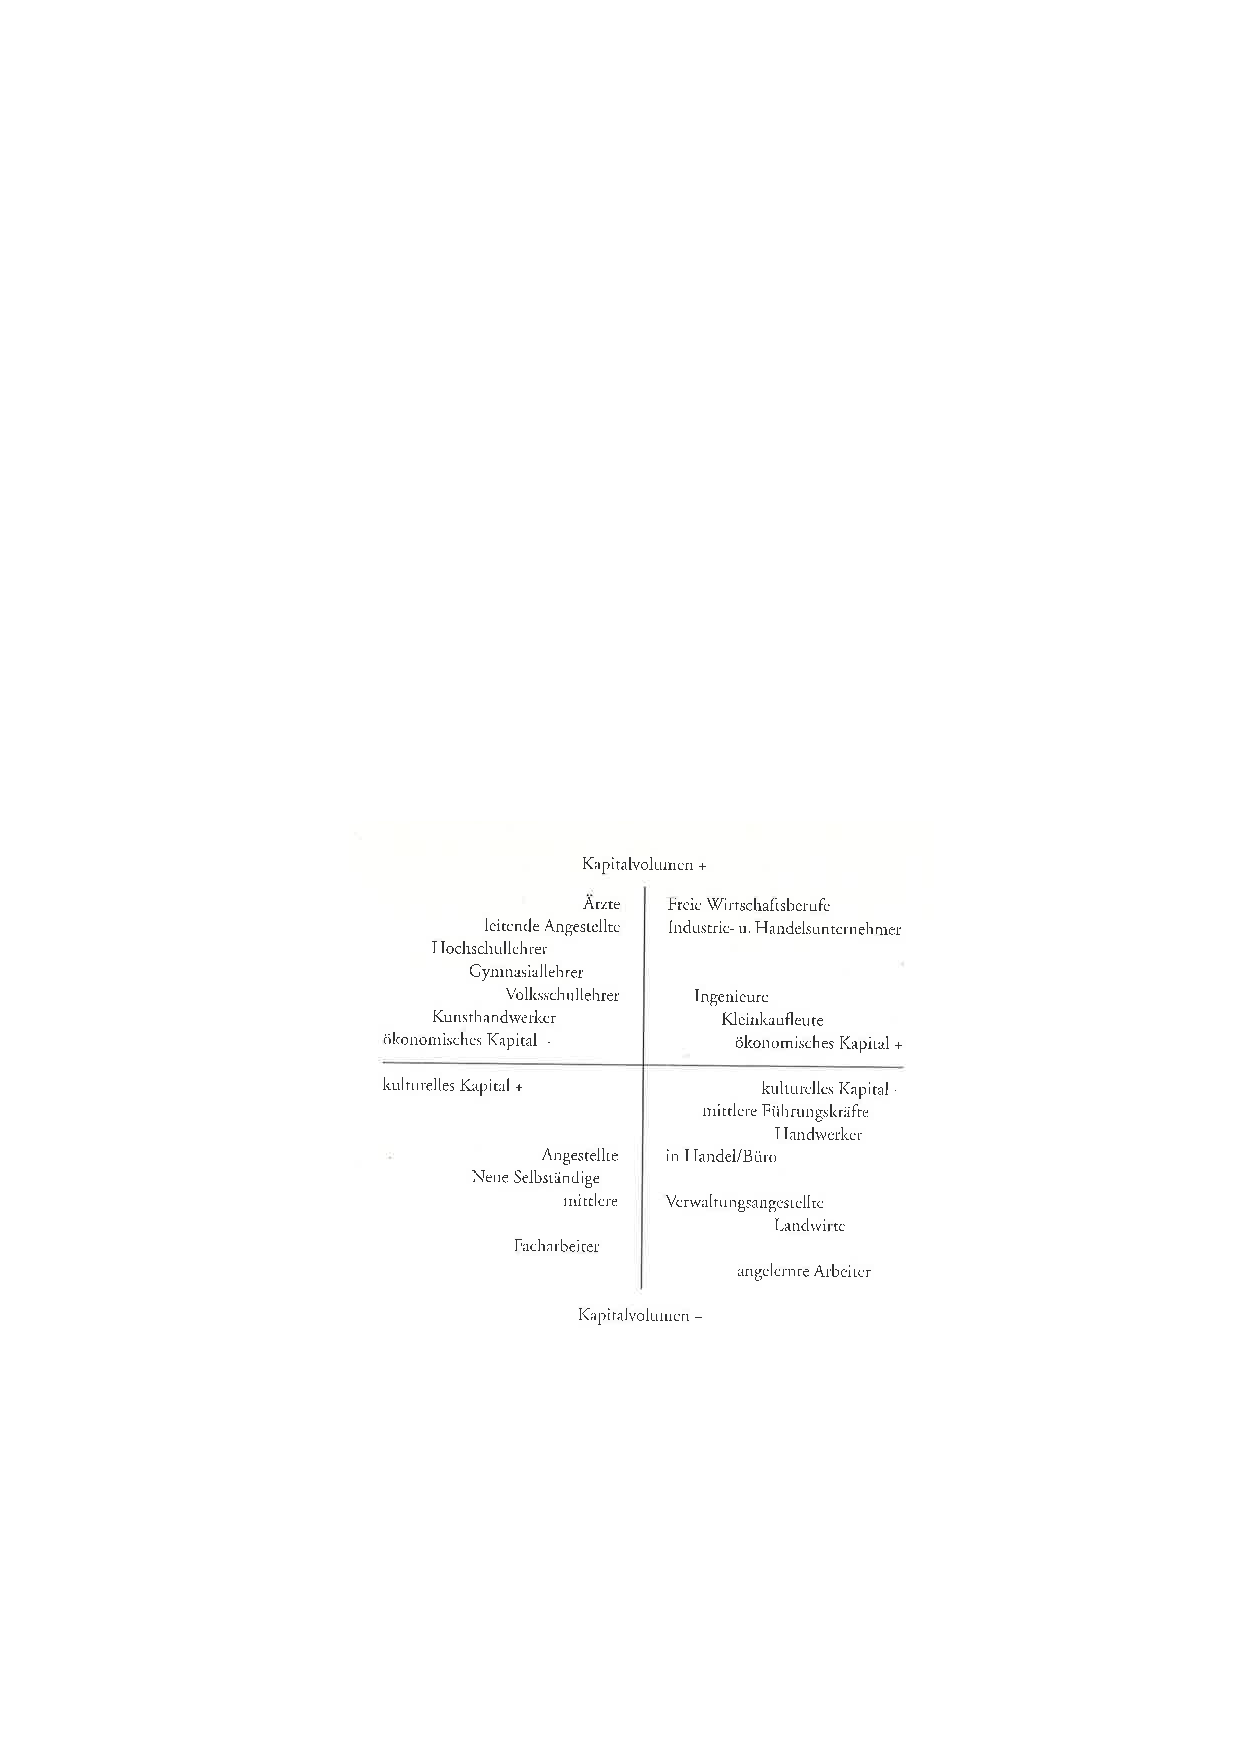
\includegraphics{Kapitalien.pdf}
	\caption{Berufsgruppen nach Kapitalsorten. Quelle: \cite[541]{joas_sozialtheorie:_2004}}
	\label{kapitalgrafik}
\end{figure}

Plastischer darstellen lässt sich dieser Zusammenhang anhand eines Beispiels. Obwohl Studierende während des Studiums meist ein geringes ökonomisches Kapital zur Verfügung haben, erwerben sie eben durch ihr Studium eine Menge an anderem Kapital: Im Laufe ihres Studiums bauen sie Beziehungen und Netzwerke auf, die Menge an sozialem Kapital steigt also. Zugleich erwerben sie eine große Menge an Wissen, einerseits Faktenwissen, andererseits auch Wissen um die Regeln in einem gewissen Feld, sie bauen also ihr kulturelles Kapital aus. Nicht zuletzt durch den Erwerb eines (Bildungs-)Titels haben sie am Ende ihres Studiums eine große Menge an Kapital angesammelt, welches sie mit dem Eintritt in die Berufswelt in ökonomisches Kapital umwandeln können.

Diese Überlegungen führt Bourdieu im Konzept des Habitus zusammen, welches wohl einen seiner meist zitierten Begriffe darstellt.

% Was interessiert? Habitus und Geschmack

\section{Habitus}
\label{habitus}
Bourdieu geht davon aus, dass allen Menschen ein spezifischer Habitus innewohnt, der in Zusammenhang mit ihrer sozialen Lage steht. Unter Habitus versteht er hier Denk-, Wahrnehmungs-, und Verhaltensschemata, die durch die Sozialisation erlernt wurden, und vermittels derer man die Welt begreift nach ihnen handelt. Joas vermerkt dazu: \blockquote[{\cite[533]{joas_sozialtheorie:_2004}}]{Unsere Körperbewegungen, unser Geschmack, unsere banalsten Deutungen der Welt werden schon frühzeitig geformt und bestimmen dann in entscheidendem Ausmaß unsere weiteren Handlungsmöglichkeiten.} Keinesfalls ist damit eine völlige Determiniertheit durch die Zugehörigkeit zu einer Klasse gemeint. \blockquote[{\cite[69]{schwingel_pierre_2009}}]{Durch die äußeren materiellen, kulturellen und sozialen Existenzbedingungen - d.h. durch die gesellschaftlichen Strukturen - und deren verinnerlichende Transformation in habituelle Denk-, Erwartungs-, und Handlungsstrukturen werden lediglich die Grenzen möglicher und unmöglicher Praktiken festgelegt, nicht aber die Praktiken an sich.}

Der Habitus legt also den Spielraum fest, innerhalb dessen sich soziale Praktiken der AkteurInnen abspielen. Auch die Art und Weise, wie bestimmte Praktiken ausgeführt werden, wird durch den Habitus bestimmt.

\blockquote[{\cite[71]{schwingel_pierre_2009}}]{[Beispielsweise] ist es keineswegs ausgeschlossen, dass (...) das von Bourdieu gerne thematisierte Kleinbürgertum sich Praktiken (etwa bestimmte prestigeträchtige Sportarten oder den Besuch von Museen) zu Eigen macht, die traditionellerweise dem Groß- bzw. Bildungsbürgertum vorbehalten sind oder waren. Doch die Art der Ausführung dieser Praktiken wird sich durch ihren spezifischen Modus operandi, hier: durch den Eifer, groß- oder bildungsbürgerliche Ziele und Standards zu erreichen, durch die Beflissenheit in der Erfüllung bürgerlicher Normen, als typisch kleinbürgerliche zu erkennen geben.}

Bourdieu zufolge sind je nach Klassenzugehörigkeit der Geschmack, und daraus folgend der Lebenstil, unterschiedlich, und dadurch auch klar zuzuordnen. 

\blockquote[{\cite[278]{bourdieu_feinen_2012}}]{Der Habitus bewirkt, daß die Gesamtheit der Praxisformen eines Akteurs (oder einer Gruppe von aus ähnlichen Soziallagen hervorgegangengen Akteuren) als Produkt der Anwendung identischer (...) Schemata zugleich systematischen Charakter tragen und systematisch unterschieden sind von den konstitutiven Praxisformen eines anderen Lebensstils.}

\section{Geschmack und Distinktion}
Aus den Ausführungen zum Habitus schon angeklungen sieht Bourdieu eine starke Verbindung zwischen der sozialen Lage und dem Geschmack. Geschmack ist hier nicht nur im engen Sinne des sensuellen Geschmackes bezogen auf Essen und Trinken, sondern im weiteren Sinne zu verstehen. So bezieht er sich explizit auf den Musikgeschmack, den Geschmack für bestimmte bildende KünstlerInnen, insofern also den Geschmack hinsichtlich der Kultur. Auch der Kleidungsstil und die Wohnungseinrichtung lassen sich Bourdieu zufolge bestimmten Berufsgruppen, Bildungsschichten, und damit in der Folge bestimmten Klassen zuordnen. \parencite[vgl.][25]{bourdieu_feinen_2012}

Bourdieu unterscheidet hierbei zwischen dem \emph{legitimen}, dem \emph{mittleren} und dem \emph{populären} Geschmack. Der \emph{legitime} Geschmack steht für Werke und Praktiken, die der Ästhetik der herrschenden Klasse entsprechen, insofern durch sie \enquote{legitimiert} werden. \parencite[vgl.][551]{joas_sozialtheorie:_2004} In der Welt der Musik stehen für ihn Werke wie Bachs \enquote{Kunst der Fuge} oder Ravels \enquote{Konzert für die linke Hand} für den legitimen Geschmack.

Indem die herrschende Klasse bestimmte kulturelle Werke oder Praktiken als \enquote{legitim} darstellt, such sie sich auch von den anderen Klassen abzugrenzen, sich von ihnen zu \emph{distinguieren}. Dieser Prozess lässt sich anhand des Opern- und Konzertbesuchs der oberen Schichten im 19. Jahrhundert veranschaulichen.

% ausführlicher darstellen: legitimen geschmack, diskurs um hohe kunst, inwiefern hängt das mit dem lebensstil zusammen. leitet über zum nächsten abschnitt

\section{Oper und Konzert - unterschiedliche Distinktionspraktiken im Fokus}
\label{operUndKonzert}

Die Oper und das Konzert sind Rezeptionsformen von Musik, die besonders im 18. und 19. Jahrhundert dem Adel und dem gehobenen Bürgertum Raum zur Distinktion gaben. Vergleicht man den Opernbesuch und den Konzertbesuch zeigt sich, dass der Akt des \enquote{Sehen und Gesehen werdens} bei der Oper stärker ausgeprägt war.

Beginnend bei der durch die Architektur der Opernhäuser angelegten Trennung der verschiedenen Klassen lässt sich erkennen, wie gut sich der Opernbesuch zur Zurschaustellung des eigenen Status eignete. Besonders die Logen waren seit jeher ein Territorium der Oberschicht: adlige oder wohlhabende Familien pachteten mitunter eine Loge für eine ganze Saison, in die sie dann Freunde und Geschäftspartner einluden. Im zweiten Rang fanden sich hauptsächlich Vertreter aus dem gehobenen Bürgertum ein, also RichterInnen, AnwältInnen und ÄrztInnen, während der dritte Rang und das Parkett hauptsächlich von Kaufleuten, LehrerInnen, Studierenden und manchmal auch Bediensteten bevölkert wurde. \parencite[vgl.][79]{muller_publikum_2014}

Auch ein Blick in Zeitungsberichte zu Opernaufführungen offenbart die Bedeutung des Opernbesuches für die oberen Schichten. Ein typischer Zeitungsbericht bestand ausschließlich aus einer Aufzählung der Personen, welche die Opernaufführung besucht hatten, \blockquote[{\cite[80]{muller_publikum_2014}}]{absteigend vom Hochadel zum Landadel, gefolgt von Parlamentariern, Militärangehörigen (...) bis hinab zu Geschäftsleuten udn bürgerlichen Mistresses und Misters.} Über die musikalische Qualität wurde hingegen nichts berichtet.

Im Gegensatz dazu hatte das Konzert einen weniger exkludierenden Charakter. Schon die Anordnung des Großteils des Publikums im Parkett, also auf gleicher Höhe, und mit mehr oder minder gleich guter Sicht auf die Bühne, eignete sich weniger, um sich von anderen Schichten abzuheben. Trotzdem lassen sich auch hier Praktiken der Distinktion entdecken. So war es in den Anfängen des Konzertwesen nicht üblich, dass mit einem Ticket für das Konzert auch eine Sitzplatzreservierung einher ging. Vielmehr gingen die KonzertbesucherInnen entweder selbst früh genug zum Konzert, oder sie sandten Bedienstete, um einen Platz zu reservieren. Die Einführung von Sitzplatzreservierungen änderte diese Praxis, und formalisierte auch die Unterschiede zwischen den verschiedenen Klassen. \parencite[30]{weber_music_2004}

\blockquote[{\cite[30]{weber_music_2004}}]{The special tickets (...) afforded people a stronger sense of social distinction.  Not only did they keep less affluent people from getting the best seats, they also defined high status in a more rigid manner than before.}

Es erscheint deutlich, dass der Opern- und Konzertbesuch für die Eliten des 19. Jahrhunderts ein wichtiger Schauplatz des öffentlichen Lebens und der Darstellungen ihrer sozialen Position und Dominanz. Auch die Dissonanzen innerhalb der Klassen, zwischen VertreterInnen der \enquote{popular music} und VerfechterInnen der \enquote{classical music} lassen sich als Kampf um den \emph{legitimen} Geschmack interpretieren. Die zunehmende Kanonisierung der Konzertprogramme gegen Ende des 19. Jahrhunderts spricht für eine Konsolidierung des Musikgeschmacks, mit welchem sich die Elite von den anderen Schichten abzuheben versuchte. \parencite[vgl.][127]{muller_publikum_2014}





\chapter{Aktuelle empirische Erhebungen zum klassischen Konzertpublikum}
Nach der ausführlichen Diskussion historischer Analysen über das Konzertpublikum wollen wir uns im Folgenden aktuellen empirischen Erhebungen widmen. Einerseits sollen die Ergebnisse zu sozioökonomischen Daten aus einer Erhebung von \textcite{de_la_motte-haber_konzertpublika_2007} diskutiert werden, andererseits wird mit dem Text von \textcite{gebesmair_grundzuge_2001} das Konzept der \enquote{Omnivores}, und damit neuere Entwicklungen des \emph{legitimen} Geschmacks diskutiert werden.

\section{Soziodemographische Befunde für das Publikum klassischer Konzerte}
In einer groß angelegten Studie untersuchte \textcite{de_la_motte-haber_konzertpublika_2007} die Konzertpublika der Gegenwart in Berlin. Mittels Fragebogen wurden insgesamt 6443 KonzertbesucherInnen von Konzerten unterschiedlichester Stilrichtungen\footnote{Zu den der Klassik zuordenbaren Konzerten gehörten in der Studie ein Konzert der Berliner Barock Solisten, ein Konzert des Klaviertrios Zacharias, ein Konzert der Berliner Philharmoniker, sowie eine Opernaufführung von Tristan und Isolde. Weiters wurden Besucher eines Konzerts der neuen Musik (musik-biennale berlin), sowie von Konzerten von Shakti und Taj Mahal, welche dem Jazz zuzordnen sind, befragt. Die anderen Konzerte gliedern sich in Konzerte der Richtungen Rock/Pop, Dance und Schlager/Volksmusik.} nach soziodemographischen Merkmalen, sowie zu bestimmten Werthaltungen, Persönlichkeitsmerkmalen, der Parteipräferenz und ähnlichem befragt. Ich werde mich im Folgenden hauptsächlich auf die soziodemographischen Daten beziehen, da diese zumindest in Ansätzen der historischen Datenlage entsprechen, und so das Aufzeigen von Kontinuitäten und Veränderungen erleichtern.

Bezogen auf die Konzertpublika von klassischen Konzerten finden sich hinsichtlich des Geschlechts keine Unterschiede. Frauen und Männer besuchen fast zu gleichen Teilen klassische Konzerte, wobei in der Kammermusik ein leichter Frauenüberhang vorherrschte, bei dem Konzert der Biennale ein leichter Männerüberhang. \parencite[vgl.][484]{de_la_motte-haber_konzertpublika_2007} Betrachtet man das Alter ergibt sich der Befund, dass die Konzertpublika der klassischen Konzerte recht breit gestreut sind. Zwar liegen die Mittelwerte der Konzerte bei knapp 50 Jahren, allerdings weisen sie alle eine große Standardabweichung von ca. 16 Jahren. Unter der Annahme einer Normalverteilung würden also ca. 68\% der BesucherInnen zwischen 34 und 66 Jahren sein. \parencite[vgl.][480]{de_la_motte-haber_konzertpublika_2007} Die Annahme der Normalverteilung ist in diesem Fall aber stark anzuzweifeln. Gerade in einer Großstadt wie Berlin, mit einer rennomierten Universität für die Ausbilung klassischer MusikerInnen, ist damit zu rechnen, dass die Studierenden auch zu klassischen Konzerten gehen. Die große Standardabweichung ließe sich zum Beispiel auch dadurch erklären, dass sich das Publikum hauptsächlich aus Personen über 66 Jahren (PensionistInnen) und Personen unter 34 Jahren (StudentInnen) zusammensetzt. Eine solche bimodale Verteilung wäre in diesem Fall sehr plausibel. Die Tatsache, dass bei Konzerten der neuen Musik 22\% der BesucherInnen Studierende waren bestärkt die Bedeutung dieser Hypothese. \parencite[vgl.][486]{de_la_motte-haber_konzertpublika_2007}

\subsection{Sozioökonomischer Status - Berufliche Stellung}
Eine aussagekräftige Variable, auch im Lichte von Bourdieus Theorien zum Geschmack ist die Bildung. Allgemein ist der Anteil an Personen mit Hochschulreife bei allen untersuchten Konzerten höher als in der Gesamtbevölkerung, auch bei Konzerten der Sparten Pop, Dance oder Schlager. Spezifisch zeigt sich aber, dass die Publika der klassischen Konzerte ein hohes Bildungsniveau haben: Fast 80\% der KonzertbesucherInnen weisen eine Hochschulreife auf. Bezieht man die Tatsache mit ein, dass ältere Personen, bedingt durch die Veränderungen des Bildungssystems, systematisch niedrigere Bildungsabschlüsse haben als junge Menschen, verstärkt sich dieser Befund noch drastisch: Im Publikum der Berliner Philharmoniker fanden sich fast fünf mal so viele Personen mit Hochschulreife wie in einer durchschnittlichen Population gleichen Alters. Die Einbeziehung dieses Kohorteneffekts setzt die klassische Musik auch stark von allen anderen Musikrichtungen, vom Jazz abgesehen, ab. Insofern scheint das klassische Konzert immer noch eine Domäne des (Bildungs-)Bürgertums zu sein. \parencite[vgl.][482]{de_la_motte-haber_konzertpublika_2007}

Die Betrachtung der beruflichen Stellung der KonzertbesucherInnen liefert weitere Daten, die die Verankerung des klassischen Konzerts in den Reihen der oberen Mittelschicht untermauern. So finden sich in den klassischen Konzerten hauptsächlich Personen aus akademisch qualifizierten, gehobenen Tätigkeiten wie HochschullehrerInnen, BeamtInnen des höheren Dienstes, NaturwissenschaftlerInnen, JuristInnen und ÄrztInnen, \textquote[{\cite[486]{de_la_motte-haber_konzertpublika_2007}}]{während dort \emph{überhaupt keine} Handwerker oder Arbeiter anzutreffen sind.} Auch die Analyse nach dem Berufsprestige (\enquote{International Socio-Economic Index of Occupational Status}) zeigt ganz deutlich, dass sich die Konzertpublika klassischer Konzerte aus Personen zusammensetzen, welche ein deutlich höheres Berufsprestige aufweisen, als alle anderen Stilrichtungen.

%%%%%%%%%%%%%%%%%%%%%%%%%%%%%%%%%%%%%%%%%%%%%%%%%%%%%%%%%%%%%%%%%%%%%%%%%%%%%%%%%%%%%%%%%%%%%%%%%%%%%%%%%%%%%%%%%%%%%%%%%%%%%%%%%%%%%%%%%%%%%%%%%%%%%%%%%%%%%%%%%%%%%%%%%%%%%%%%%%%%%%%%%%%%%%%%%%%%%%%%%%%%%%%%%%%%%%%%%%%%%%%%%%%%%%%%%%%%%%%%%%%%%%%%%%%%%%%%%%%%%%%%%%%%%%%%%%%%%%%%%%%%%%%%%%%%%%%%%%%%%%%%%%%
$-->$ Grafik der Korrespondenzananlyse hier rein
%%%%%%%%%%%%%%%%%%%%%%%%%%%%%%%%%%%%%%%%%%%%%%%%%%%%%%%%%%%%%%%%%%%%%%%%%%%%%%%%%%%%%%%%%%%%%%%%%%%%%%%%%%%%%%%%%%%%%%%%%%%%%%%%%%%%%%%%%%%%%%%%%%%%%%%%%%%%%%%%%%%%%%%%%%%%%%%%%%%%%%%%%%%%%%%%%%%%%%%%%%%%%%%%%%%%%%%%%%%%%%%%%%%%%%%%%%%%%%%%%%%%%%%%%%%%%%%%%%%%%%%%%%%%%%%%%%%%%%%%%%%%%%%%%%%%%%%%%%%%%%%%%%%%

Die im ersten Teil der Arbeit behandelte Genese des Konzertes scheint sich auch noch in der heutigen Zeit zu reproduzieren. Genauso wie in den Anfängen des bürgerlichen Konzertes sind es Personen der oberen Mittelschicht, die sich für klassische Musik interessieren. Die Bedeutung der klassischen Musik für die Herausbildung eines \emph{legitimen} Geschmackes, und somit zur Distinktion der Oberschicht scheint aber abgenommen zu haben. Das Konzept der \enquote{Omnivores} unterstreicht diese Hypothese.

\subsection{Veränderter Musikgeschmack der Eliten}
Neben der nach wie vor starken Verankerung der klassischen Musik in der oberen Mittelschicht scheint die Bedeutung der klassischen Musik als Mittel zur Distinktion abzunehmen. \textcite{gebesmair_grundzuge_2001} rezipiert hier vor allem das von \textcite{peterson_understanding_1992} eingeführte Konzept der \enquote{Omnivores}, zu Deutsch: Allesfresser. Während Bourdieu noch stark die Bedeutung des hochkulturellen Geschmacks als \emph{legitimer} Geschmack betont, scheint dieser nicht mehr auszureichen, um als zur herrschenden Klasse zugehörig zu gelten. Größere Bedeutung erlangt ein möglichst breiter Geschmack, der eben nicht, wie bei Bourdieu, in starker Abgrenzung zum populären Geschmack besteht. 

\blockquote[{\cite[252]{peterson_understanding_1992} zitiert nach \cite[206]{gebesmair_grundzuge_2001}}]{In effect, elite taste ist no longer defined simply as the expressed appriciation of the high art forms and a corresponding moral disdain of, or patronizing tolerance for, all other aesthetic expressions. (...) Because status is gained by knowing about, and participating in (that ist to say, by consuming) many if not all forms, the term omnivore seems appropriate for those at the top of the emerging status hierarchy}



% % Begründung für die These, dass Konzert früher stärkere Repräsentationsfuktion hatte...
% % der folgende Teil passt besser zur soziologischen Analyse
% Konzert als Mittel zur Distinktion
% Aufzählung der Gäste (müller 91)
% Publizierung der Mitgliederlisten


\chapter{Resümee}
Das Ziel der Arbeit, einen Überblick über aktuelle Erhebungen zu den Konzertpublika klassischer Konzerte zu gewinnen, der in Verbindung mit der historischen Genese des Konzertes steht. Ausgehend von frühen Formen des Zusammenschlusses musikliebender Personen, den Konzertvereinigungen, entwickelte sich im Europa des 19. Jahrhunderts ein reges Musikleben. Es entstanden Konzertserien, neue Aufführungsorte, und die Konzerte zogen mit der Zeit immer mehr Menschen an. Trotzdem gelang es der Elite sich abzugrenzen. Durch die Einführung von Sitzplatzreservierungen und ähnlichen Praktiken blieb das Konzert eine Domäne der Oberschicht. Die Zusammensetzung ebendieser Oberschicht war im Laufe des 19. Jahrhunderts aber einer Veränderung unterworfen. Konstituierte sich das Publikum zum Beginn des 19. Jahrhunderts aus dem Adel und hohen Vertretern des Klerus, übernahm im Lauf des Jahrhunderts das aufstrebende Bürgertum die Oberhand über den Konzertbetrieb, und somit auch über die Definition des legitimen Geschmacks. Befeuert durch die wirtschaftlichen Veränderungen gelang immer mehr BürgerInnen die Etablierung in einer vormals dem Adel zugeordneten Kunstrichtung.

Die sozialen Strukturen, welche für das Konzertpublikum des 19. Jahrhunderts prägend waren, lassen sich auch in den Publika der heutigen Konzerte nachzeichnen. So rekrutiert sich das heutige Publikum weiterhin aus der (bildungs-)bürgerlichen Mittel- bis Oberschicht. ÄrztInnen, JuristInnen, Natur-und GeisteswissenschafterInnen, BeamtInnen des höhere Dienstes, also vornehmlich Personen mit einer hohen Bildung und einem hohen Berufsprestige, um mit Bourdieu zu sprechen also Personen, mit hohem kulturellen Kapital bilden weiterhin den Kern des klassischen Konzertpublikums.

Allerdings scheint die Bedeutung der klassischen Musik als Distinktionsmerkmal abgenommen zu haben. Der Habitus der Oberschicht hat nur mehr wenig mit dem Habitus des/der großbürgerlichen Konzertgehers/geherin gemein. Um in den oberen sozialen Schichten zu reüssieren, ist ein möglichst breiter Geschmack vonnöten, die reine Fixierung auf die Hochkultur reicht nicht mehr aus, um Kraft seines Habitus' der Oberschicht zugeordnet zu werden. Insofern scheint die Entwicklung des Konzertpublikums einen, für die Interpreten, erfreulichen Weg genommen zu haben: Wiewohl der Besuch eines Konzertes für bestimmte Gruppen sicherlich noch \enquote{zum guten Ton gehört} scheint doch das inhaltliche Interesse an der Musik heute größer, als zur Anfangszeit des \enquote{bürgerlichen Konzertes}.



\printbibliography[filter=LV]
\printbibliography[heading=IQ, filter=IQ]
\end{document}

